\chapter{High-throughput smFRET}
\label{chpt:ht-smFRET}

Diffusion-based \ac{smFRET} measurements offer the advantage of minimal perturbation to the studied molecule, as compared to measurements on immobilized molecules~\cite{rhoades_PNAS_2003,selvin_CSHLP_2008,cohen_OE_2008}.
The ability to study small volumes of low-concentration samples is particularly valuable in various applications, such as those in diagnostics, where patient samples are often limited, and target molecules may exist in very low abundance. 

However, there are limitations to diffusion-based measurements.
To ensure the identification of each molecular transit as a distinct burst of photons, only one molecule may pass through the excitation-detection volume at a time.
For this reason, these experiments are usually constrained to concentrations $\leq$ 100 pM.
This limitation poses challenges in collecting a sufficient number of bursts for robust statistical analysis. 
Nonetheless, solution-based single-molecule FRET remains a valuable tool, especially when sensitivity to low concentrations and minimal perturbation are critical.

In practice, this means that single-molecule measurements can extend over minutes to hours, which limits the application of \ac{smFRET} to equilibrium reactions unless complemented by other techniques like microfluidic mixers or trapping methods. 
Even with these enhancements, gathering statistically significant data requires extended acquisition times. 
This is because recording single-molecule data sequentially at each time point, as seen in a mixer, or capturing enough individual molecule time-trajectories, as encountered in trapping, can be time-consuming. 
Parallel or multiplexed acquisition methods are a promising solution to challenges associated with single-molecule detection,  and in the case of diffusion-based measurements also prevent potential immobilization-related artifacts.
These approaches hold the potential to broaden the applicability of \ac{smFRET}, allowing for rapid non-equilibrium kinetic studies and eventually highly sensitive clinical diagnostics.

Expanding upon the recent advancements in single photon avalanche diode (\ac{SPAD}) arrays, we have successfully showcased parallel detection of single molecules and achieved freely diffusing \ac{HT-smFRET}. 
This was accomplished through the iterative design of experimental setups where multiple excitation spots in the sample align with the geometry of the detector array. 

\section{Custom silicon SPAD arrays}
\label{sec:SPAD_intro}

In this work, we employed custom epitaxial silicon \ac{SPAD} arrays that were meticulously designed and manufactured by the \ac{SPAD} lab at \ac{POLIMI} in Milan, Italy~\cite{ghioni_JSTQE_2007,gulinatti_JMO_2012,gulinatti_SPIE_2013}. 
The state-of-the-art detector module comes equipped with \ac{iAQC}, engineered to rapidly reset the \ac{SPAD}s following the creation of an avalanche triggered by the absorption of an incoming photon.

Additionally, these modules are endowed with timing electronics that enable the precise counting of single photons. 
In some cases, they also feature \ac{TCSPC} electronics, which improve the time resolution of single-photon timing to approximately 50~ps~\cite{ingargiola_SPIE_2017}.

Over the past two decades, alternative \ac{SPAD} array designs have emerged, utilizing standard complementary metal oxide semiconductor (\ac{CMOS}) fabrication technology~\cite{bruschini_SPIE_2017}. 
These designs offer the advantage of larger scales, with some arrays comprising over 100,000 \ac{SPAD}s. 
This scalability is particularly advantageous for wide-field imaging techniques like \ac{FLIM}~\cite{gyongy_IEEETED_2018, ulku_JSTQE_2019} or \ac{HT-FCS}~\cite{buchholz_BJ_2018}.

However, based on experience~\cite{ colyer_SPIE_2011}, \ac{CMOS} \ac{SPAD} arrays tend to exhibit lower \ac{PDE} and generally higher \ac{DCR}s when compared to custom silicon \ac{SPAD} detectors~\cite{ghioni_JSTQE_2007, michalet_JSTQE_2014}. 
As a result, they are a poor choice for the detection of freely diffusing single molecules.

However, due to the rapid pace of technological innovation in this field, this statement regarding \ac{SPAD} array technology will likely become quickly outdated. 
In addition to the differences mentioned, custom technology \ac{SPAD}s offer the advantage of manufacturing larger individual \ac{SPAD}s while maintaining low \ac{DCR}s. 
This characteristic simplifies the precise optical alignment of the setup, making custom \ac{SPAD} arrays particularly well-suited for single-molecule fluorescence studies.

\section{HT-smFRET-PAX setup description}
\label{sec:smFRET-PAX_setup}

\begin{figure}
\centering
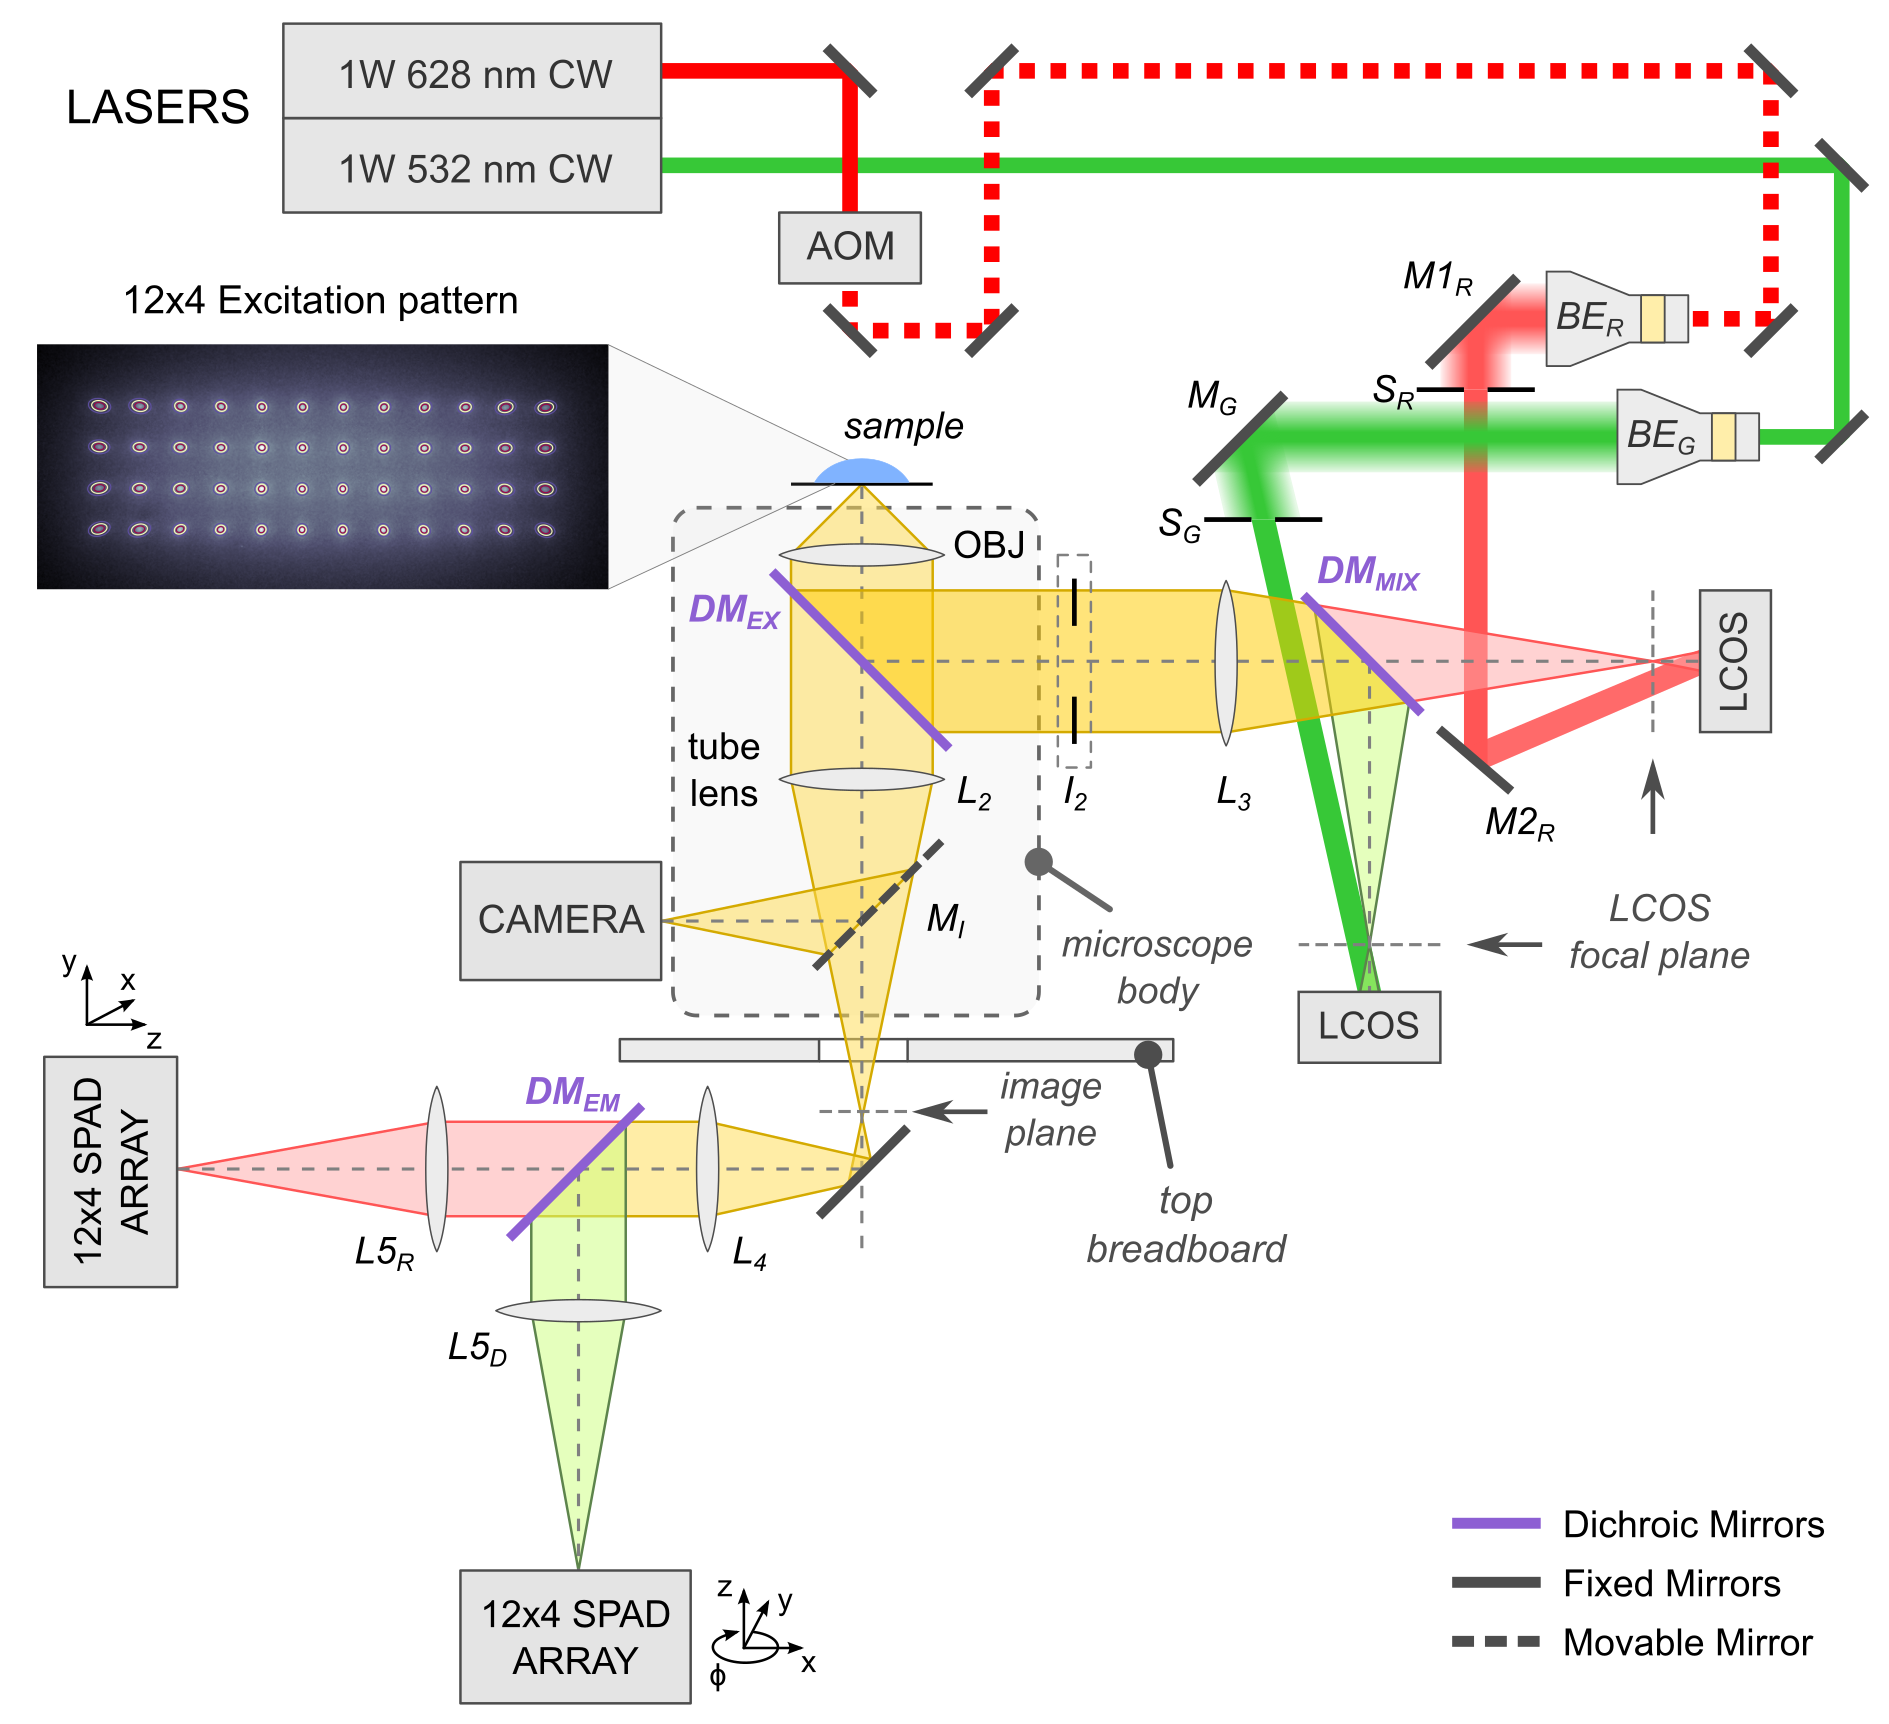
\includegraphics[width=0.7\linewidth]{chapters/figures/design_multispot_LCOS_camera_SPAD.png}
\caption{\label{fig:setup} 48-spot PAX design schematic. 
The two \ac{CW} lasers and \ac{SPAD} arrays are fixed to a floated optical table. 
Periscopes are used to bring the beams to the optical breadboard supporting the microscope and \ac{LCOS-SLM}s. 
Two beam expanders, mirrors, one dichroic mirror, and one lens are used to steer the beams to their respective SLMs, form spot arrays, and relay them to the back of the back of the microscope objective lens.
The microscope side port is used to monitor the beam pattern using a \ac{CMOS} camera (an example of which is shown on the left), while the bottom port is used to send the fluorescence signal to the two \ac{SPAD} arrays via relay lenses, a dichroic mirror, and emission filters. 
A detailed description can be found in the text.
Reprinted from Ingargiola \textit{et al.}~\cite{ingargiola_JCP_2018}.}
\end{figure}

The concept of a multispot setup involves replicating the conventional confocal arrangement of an excitation spot and detector, with the requirement that each confocal spot in the sample corresponds to one \ac{SPAD} in the \ac{SPAD} array. 
Note that an individual \ac{SPAD} is sometimes referred to in this work as a \enquote{pixel}, \enquote{channel}, or \enquote{spot}.
Several methods can be employed to achieve this, including using physical lenslet arrays, which we initially explored~\cite{colyer_SPIE_2010}, or diffractive optical elements~\cite{gosh_JBO_2005, krmpot_SPIE_2015}. 
However, these approaches have limitations, such as fixed spot geometries and potential aberrations that must precisely match the pattern of the \ac{SPAD} array in the emission path. 
Achieving this alignment requires meticulous magnification adjustments and cumbersome alignment steps, including rotational adjustments.

For these reasons, we opted for a more flexible, though somewhat more expensive solution involving the use of programmable liquid crystal on silicon spatial light modulators (\ac{LCOS-SLM}s). 
This approach has been detailed in previous work from the Weiss Lab~\cite{colyer_BOE_2010,ingargiola_SPIE_2013,ingargiola_PLOS1_2016,ingargiola_JCP_2018}.

These devices can be employed in either direct space~\cite{wang_OE_2005} or reciprocal space~\cite{dufresne_RSI_2000}, as utilized in holography. 
The direct space approach offers the advantage of simple and real-time modification of the pattern. 
The \ac{LCOS-SLM}s are capable of generating relatively uniform spots over the typical field of view of a high \ac{NA} objective lens~\cite{michalet_PRSB_2013}.

Alternatively, a line or sheet illumination pattern can be used, relying on out-of-focus light rejection by the geometry of the detector array itself (Fig.~\ref{fig:multispot_geometries}B). 
We demonstrated this with a linear array~\cite{ingargiola_SPIE_2017}, and others demonstrated it with a 2D array~\cite{buchholz_OE_2012}. 
Although the latter demonstration was not in the context of single-molecule experiments, the concept is applicable to \ac{smFRET}.

However, these approaches have drawbacks, including increased background signal and inefficient excitation power distribution due to the absence of focused excitation light. 
Additionally, there is a concern about increased photobleaching due to the larger volume of the sample where fluorophore excitation occurs. 
This concern can be mitigated by using flowing samples, such as when combining a multispot setup with microfluidics, as discussed later in Section~\ref{sec:smFRET_microfluidics}.

In our first iteration of a \ac{HT-smFRET} setup, we developed an 8-spot confocal microscope using an \ac{LCOS-SLM} optically conjugated to a single linear 8-\ac{SPAD} array. 
The 8-spot setup (Fig.\ref{fig:multispot_geometries}A) employed a single \ac{CW} laser and was used to demonstrate single-molecule detection~\cite{colyer_BOE_2010} capabilities as well as \ac{HT-FCS}. 
We later added a second linear 8-\ac{SPAD} array to the setup to enable two-color, 8-spot \ac{smFRET} measurements~\cite{ingargiola_PLOS1_2016}. 
Both setups used a 532~nm high-power 68~MHz pulsed laser for historical reasons, although we could not take advantage of the 8~ps pulsed laser excitation with these \ac{SPAD} arrays. 
This configuration led to the development of a number of analysis tools allowing pooling of data acquired from separate spots for increased statistics (see Section~\ref{sec:analysis}).

\begin{figure} 
\centering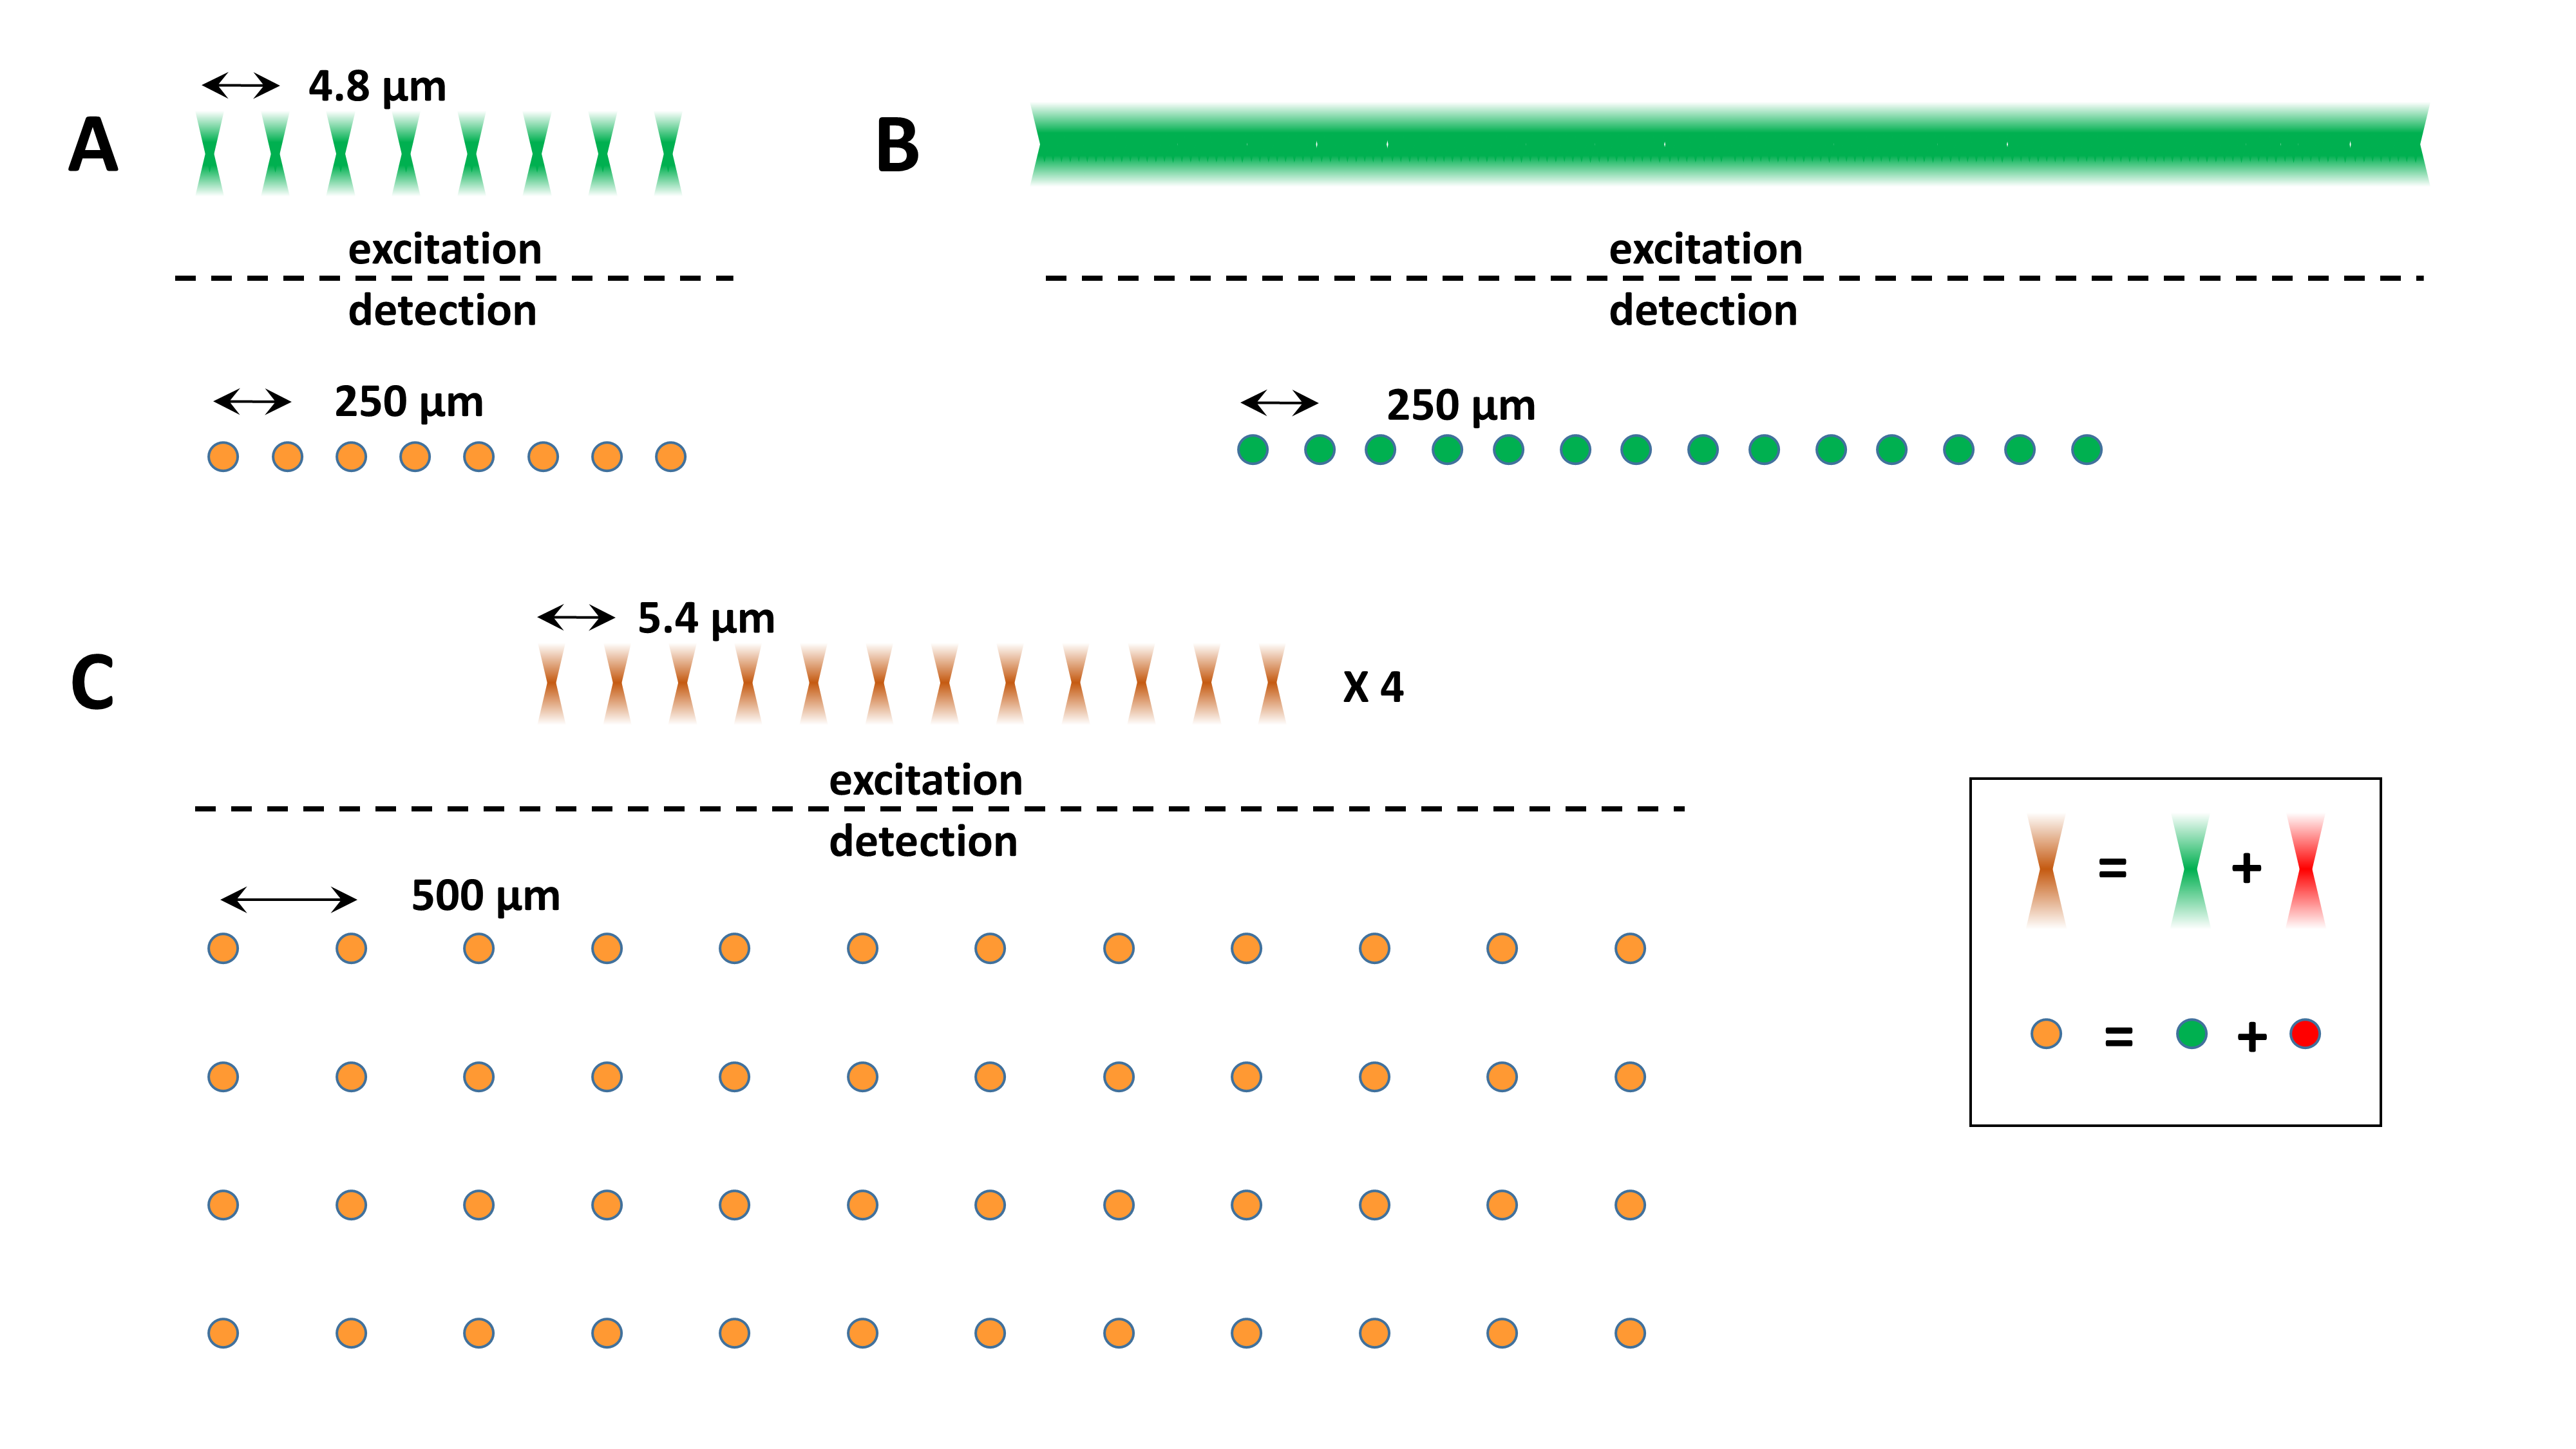
\includegraphics[width=\textwidth]{chapters/figures/multispot_geometries.png}
\caption{\label{fig:multispot_geometries} Different excitation and \ac{SPAD} array geometries used in this work.
A) Linear 8-spot and 8-\ac{SPAD} array configuration. 
The 532~nm laser used in this setup was a high-power (1~W) ps-pulsed laser (68~MHz).
The setup was initially equipped with a single \ac{SPAD} array (single color detection: green), and later upgraded with a second linear 8-\ac{SPAD} array (red + green, represented in orange). 
The physical separation between excitation spots in the sample was $4.8~\mu$m (top)~\cite{colyer_BOE_2010}, matching (after magnification) the $250~\mu$m pitch of the \ac{SPAD}s in the array (\ac{SPAD} diameter: $50~\mu$m, bottom).
B) A linear illumination pattern created with a cylindrical lens, using the same high-power laser as in A was used to excite the fluorescence of samples. 
A linear 16-\ac{SPAD} array (pitch: $250~\mu$m, diameter: $50~\mu$m) connected to a \ac{TCSPC} module was used to collect the emitted light from the conjugated spots in the sample~\cite{ingargiola_SPIE_2016}.
C) Two patterns of $12\times4$ spots were generated in the sample by two high power (1~W) lasers (532~nm and 635~nm) and their associated \ac{LCOS-SLM}s. 
The $5.4~\mu$m distance between neighboring spots, matched, after magnification, the $500~\mu$m distance between \ac{SPAD}s in the corresponding two $12\times4$ \ac{SPAD} arrays 
(\ac{SPAD} diameter: $50~\mu$m)~\cite{ingargiola_JCP_2018}.
Reprinted from Segal \textit{et al.}~\cite{segal_methods_2019}.
}
\end{figure}

Our next effort at building a \ac{HT-smFRET} setup utilized a larger linear 32-\ac{SPAD} array equipped with \ac{TCSPC} readout electronics, again developed for us by \ac{POLIMI}~\cite{cuccato_IEEEPJ_2013}.
We employed a 532~nm 86~MHz pulsed laser along with a simplified excitation optical setup. 
This setup featured a cylindrical lens that was optically aligned with the back focal plane of the microscope objective lens, resulting in a line illumination pattern, as opposed to the use of an \ac{LCOS-SLM}~\cite{ingargiola_SPIE_2017} (Fig. \ref{fig:multispot_geometries}B). 
The 32-spot \ac{smFRET} setup demonstrated that time-resolved information, such as fluorescence lifetime decays, from multiple spots, could be pooled together to accelerate data acquisition, as previously demonstrated for counting applications using \ac{CW} excitation with the 8-spot setup.

Our next iteration of the \ac{HT-smFRET} setup used an even larger $12\times4$ \ac{SPAD} array developed by \ac{POLIMI}~\cite{gulinatti_SPIE_2012, ingargiola_JCP_2018} (Fig. \ref{fig:multispot_geometries}C). 
The 48-spot setup was designed to improve throughput by expanding on the number of confocal spots.
In addition, we added two \ac{CW} lasers and two \ac{LCOS-SLM}s for the excitation of donor and acceptor dyes.
The addition of a second laser addressed limitations with single-laser excitation.
Rather than implementing \ac{ALEX}, which would require two \ac{AOM}s, we used a single \ac{AOM} to modulate the acceptor excitation only, see Section~\ref{sec:PAX_intro} for more details on this on \ac{PAX}.

Comparison of the 48-spot smFRET-PAX microscope to a standard single-spot ALEX microscope demonstrated that there was no difference in the quality of the data~\cite{ingargiola_JCP_2018}. 
However, there was a notable increase in throughput, approximately proportional to the number of \ac{SPAD}s as expected. 
This suggests that the multispot smFRET-PAX setup is a powerful tool for \ac{HT-smFRET} experiments, allowing for the simultaneous analysis of multiple samples or conditions. 
A schematic of the 48-spot setup is presented in Figure~\ref{fig:setup}.
In addition, Figure~\ref{fig:setup_photos} presents detailed photos of the excitation and emission paths.

\begin{figure}
\centering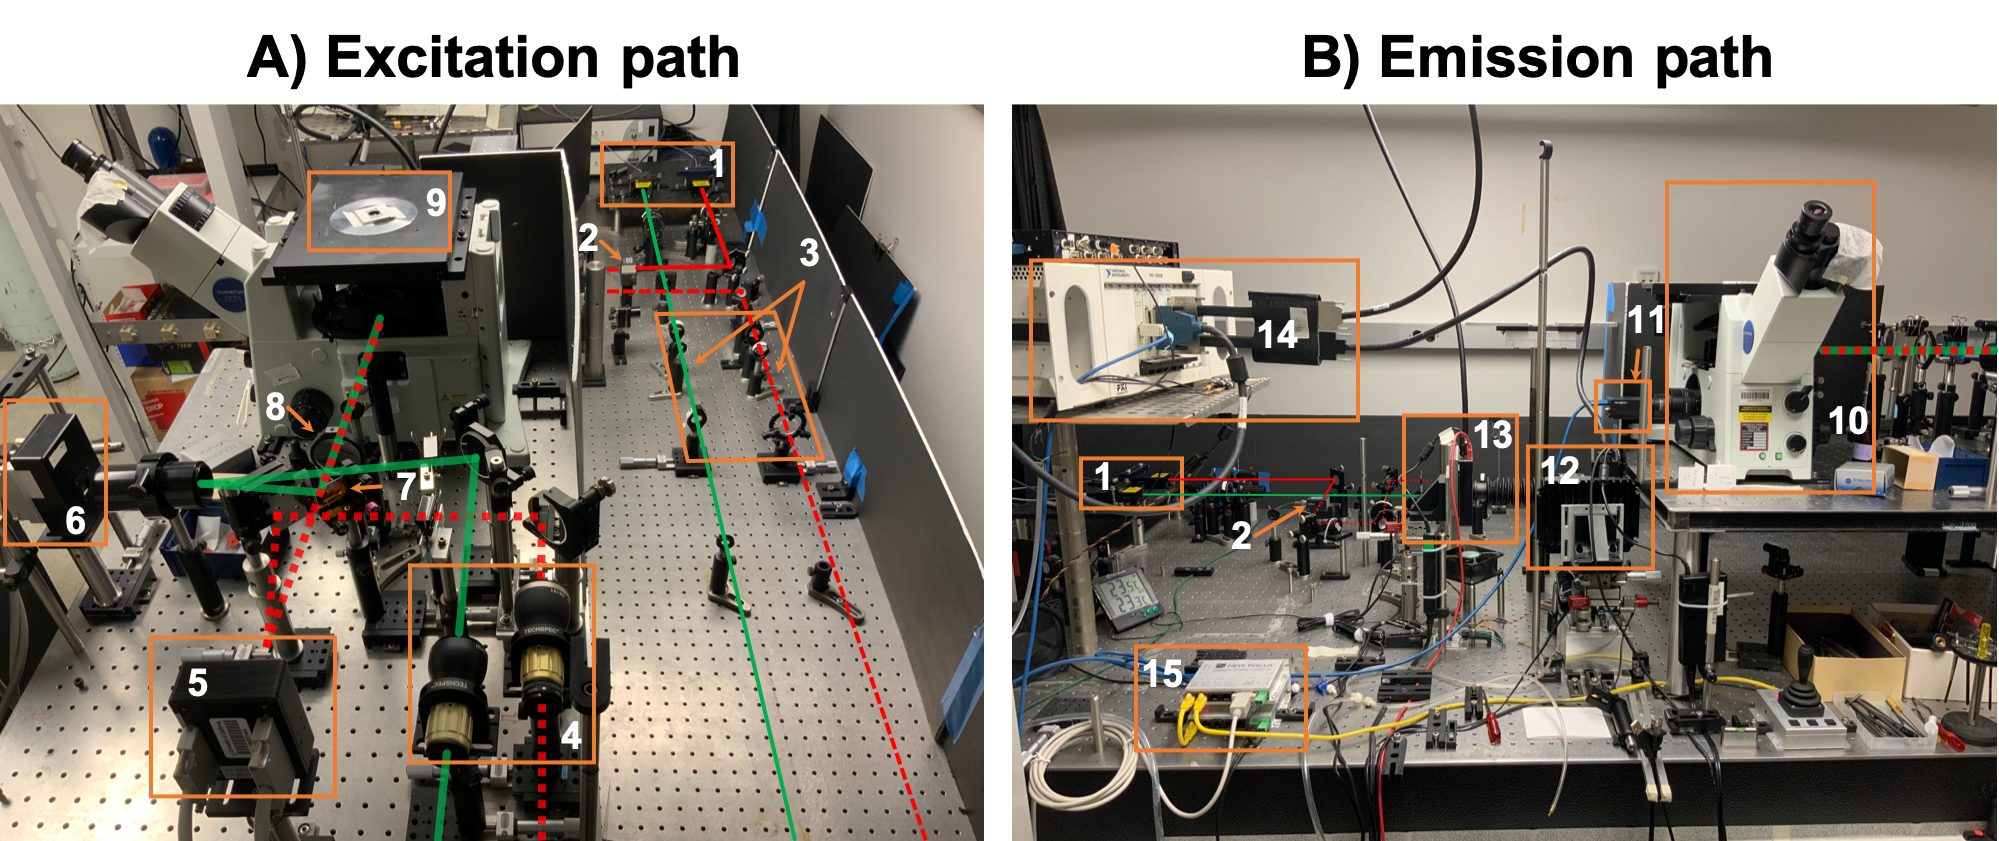
\includegraphics[width=1.0\linewidth]{chapters/figures/setup_photos.png}
\caption{\label{fig:setup_photos} Photographs of the 48-spot setup.
A) The excitation path consists of two 1~W \ac{CW} lasers (1). 
Alternation of the red laser by the \ac{AOM} (2) is indicated by red dashes. 
The lasers pass through a set of beam-expanding lenses (3) followed by a second beam expansion (4) once on the upper breadboard.
Both lasers are phase modulated by separate green (5) and red (6) \ac{LCOS-SLM}s and the resulting beamlets are combined with a mixing dichroic (7) and recollimated by a recollimating lens (8) before entering the microscope body (10). 
B) Emission path optics showing the \ac{CMOS} camera (11) attached to the top side-port for alignment and the bottom path relaying the emitted fluorescence to the green (12) and red (13) \ac{SPAD} arrays. 
Fluorescence emission is spectrally separated by a dichroic mirror and further filtered with emission filters (not visible), before being imaged onto two $12\times4$ \ac{SPAD} arrays (12 and 13)  mounted on micro-positioning stages powered by two micro-positioning drivers (15).
The single-photon pulses from the \ac{SPAD} arrays are sent to a programmable counting board (14) connected to the acquisition computer (not shown).
Reprinted from Segal \textit{et al.}~\cite{segal_methods_2019}.
}
\end{figure}

\subsection{Excitation path optics}
\label{sec:excitation_optics}

In the \ac{PAX} setup, the red laser is modulated by an \ac{AOM}, while the green laser excitation remains continuous. 
Both laser beams undergo expansion using Keplerian telescopes, as shown in Figure~\ref{fig:setup_photos}A(3). 
Subsequently, two periscopes elevate the laser beams to a breadboard where the microscope body is located. 
To ensure uniform illumination and coverage of the \ac{LCOS-SLM} pattern, the laser beams undergo a second expansion, as shown in Figure~\ref{fig:setup_photos}A(4). 

\subsection{Phase modulation by LCOS-SLMs}
\label{sec:LCOS}

In both the 8-spot and 48-spot setups, we created the lenslet pattern using the \ac{LCOS-SLM}, with each spot being optically matched to a specific \ac{SPAD} pixel. 

In the 48-spot setup, two \ac{LCOS-SLM}s were employed to independently produce patterns for each excitation wavelength. 
The patterns were controlled through phase modulation of the incoming laser wavefront, as detailed in previous work~\cite{ingargiola_PLOS1_2016, colyer_BOE_2010}. 
This phase modulation operates in direct space rather than Fourier space and replicates the phase profile of a microlens (lenslet) array.
This approach closely resembles direct-space modulation using an altered spatial arrangement of the phase pattern on the \ac{LCOS-SLM}, which has also been demonstrated for multi-confocal \ac{FCS}~\cite{kloster-landsberg_RSI_2013}.

To generate these spots using the \ac{LCOS-SLM}s, we employed two 8-bit encoded phase images, each with dimensions of $800\times600$ pixels. 
These phase images were controlled by a custom LabVIEW program, which computed the phase pattern based on user inputs and supported automated pattern scanning, as described in our previous work~\cite{ingargiola_JCP_2018}. 
The code for our custom tool is available in the \texttt{LCOS\_LabVIEW} repository on GitHub (\href{https://github.com/multispot-software/LCOS_LabVIEW}{link}).

When aligned correctly, the excitation spots converge at the sample plane. 
The lenslet array is focused at a focal length specified by the user, positioned 3-4~cm from the \ac{LCOS-SLM} surface, as depicted in Figure~\ref{fig:LCOS_params}. 

The pattern can be adjusted by changing its center position, rotation, and X and Y pitch independently, corresponding to shifting, rotating, or scaling the lenslet array. 
This adjustment is facilitated using the \texttt{LCOS\_LabVIEW} software, where both the center, pitch, and rotation of each pattern can be modified (Figure~\ref{fig:LCOS_params}, panels B and C).

\begin{figure}
\centering
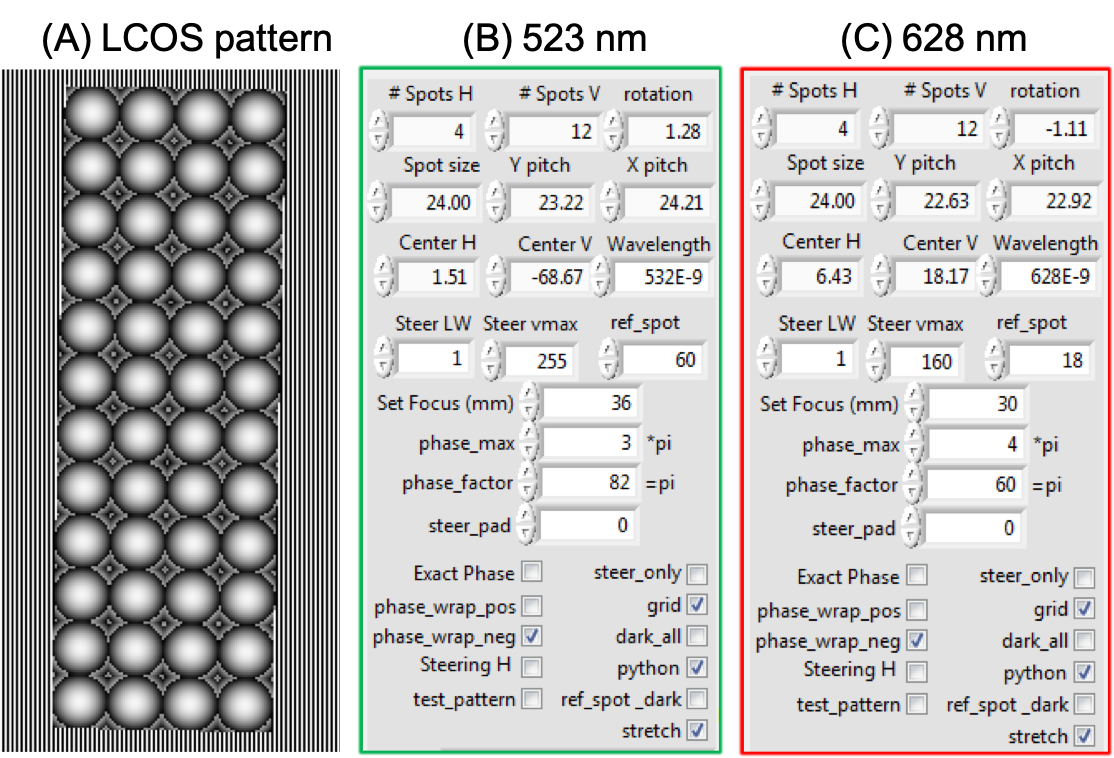
\includegraphics[width=\linewidth]{chapters/figures/LCOS_GUI.png}
\caption{\label{fig:LCOS_params} Pattern generation
using two independent \ac{LCOS-SLM}s.
Focal lengths and beam-steering parameters differ for the two laser excitations.
Adjustable parameters include number of spots, spot size, degree of rotation, pitch in X- and Y-directions, and pattern center (H, V) defined in \ac{LCOS-SLM} units. 
During alignment, these parameters are optimized using the \texttt{LCOS\_pattern\_fitting} notebook
(\href{https://github.com/tritemio/48-spot-smFRET-PAX-analysis/tree/master/alignment/2017-04-28/pattern_profiling}{link}).
(A) \ac{LCOS-SLM} generated $12\times4$ lenslet array 
surrounded by a periodic beam-steering pattern (shown for the green laser only). 
(B) and (C) show experimentally derived \ac{LCOS-SLM} parameters for the spots and beam-steering patterns of the green (532~nm) and red lasers (628~nm) respectively.
Reprinted from Segal \textit{et. al.}~\cite{segal_methods_2019}}.
\end{figure}

The dimensions of the spots are influenced by several factors, including the configuration of the \ac{SPAD} arrays, the $83\times$ reduction in size in the excitation path, and the $90\times$ enlargement in the emission path ($90\times = 60\times1.5$). 
The spot size in the sample plane, approximately $5.4~\mu$m, is determined by the pitch between adjacent \ac{SPAD}s ($500\mu$m) divided by the magnification in the emission path (approximately 90x). 
This translates to a lenslet pitch on the \ac{LCOS-SLM} of about $463~\mu$m or roughly $23.1$ \ac{LCOS-SLM} pixels. 
During alignment, the pitch is precisely adjusted to accommodate the specific demagnification in the excitation path by making minute shifts in the pattern in terms of \ac{LCOS-SLM} pixel units.

Additionally, the lenslet arrays have distinct focal lengths, with the green pattern having a focal length of 36~mm and the red pattern 30~mm. 
This difference in focal lengths is intentionally chosen to compensate for the variations in the size of the \ac{PSF} of the 532~nm and 628~nm wavelengths.

Figure~\ref{fig:pattern_profile} displays the excitation patterns for the green and red lasers, which were visualized using a camera with samples of high-concentration ATTO550 (Fig.~\ref{fig:pattern_profile}A) and ATTO647N (Fig.~\ref{fig:pattern_profile}B) dyes. 
During the alignment process, the patterns were centered on the optical axis to maximize their overlap.
The degree of overlap between the two excitations was quantified by fitting the peak position and Gaussian waist of each spot (Fig.~\ref{fig:pattern_profile}C). 
For in-depth details regarding the analysis, please refer to the \texttt{pattern\_profiling} alignment notebook, which can be found at this \href{https://github.com/tritemio/48-spot-smFRET-PAX-analysis/tree/master/alignment}{link}~\cite{ingargiola_JCP_2018}.

\begin{figure}
\centering
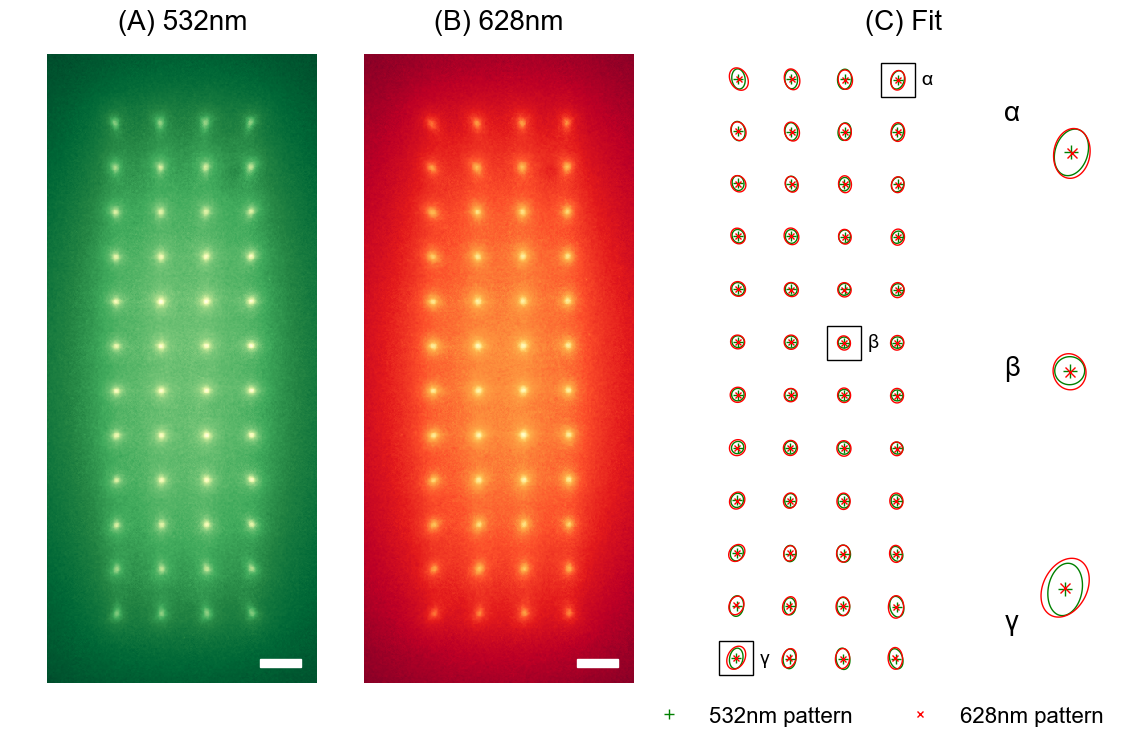
\includegraphics[width=1.0\linewidth]{chapters/figures/2017-04-28_conf9_G_conf14_R_green_red_pattern_and_fit.png}
\caption{\label{fig:pattern_profile} $12\times4$ pattern generated by the two independent \ac{LCOS-SLM}s. 
The elliptical shape and tilt of the Gaussian fits are due to residual optical aberrations. 
(A) Green (532~nm) $12\times4$ spot pattern. 
(B) Red (628~nm) $12\times4$ spot pattern. 
(C) To assess the alignment of the $12\times4$ patterns, each spot in the two images is fitted  with a tilted 2D Gaussian function. 
The degree of overlap of green and red spots is determined by comparing the peak positions (cross and star) and the outline of the Gaussian waist (green and red ovals) of each green and red spot. 
Panels (A) and (B): images of a 100~nM mixture of ATTO~550 (green) and ATTO~647N (red) dyes, acquired separately with a CMOS camera installed on the microscope side port. 
Rightmost panel: $\alpha, \beta,$ and $\gamma$ are close-ups of 3 representative spots in the $12\times4$ array. 
Scale bars = $5~\mu$m. 
Reproduced from Ingargiola \textit{et al.,} 2018~\cite{ingargiola_JCP_2018}.
}
\end{figure}

To modify the lenslet focal length, it is necessary to adjust the distance between the $L3$ lens (\ref{fig:setup}) and the \ac{LCOS-SLM} to maintain the focal plane at the correct distance. 
The \ac{LCOS-SLM} region surrounding the $12\times4$ pattern can receive light, potentially leading to stray wide-field excitation and an increase in background signals. 
To mitigate this, we fill the unused \ac{LCOS-SLM} area with a \enquote{beam steering} pattern, which consists of a periodic pattern in one direction, described in more detail in Section~\ref{sec:background_suppression}. 

It is worth highlighting a fundamental difference in our approach compared to Kloster-Landsberg's~\cite {kloster-landsberg_RSI_2013} method. 
In our setup, different portions of the \ac{LCOS-SLM} are allocated to different spots, while Kloster-Landsberg's method uses a much longer focal length to create a single phase pattern that combines contributions from all spots~\cite{kloster-landsberg_RSI_2013}. 
A detailed experimental comparison to assess the relative strengths of these two approaches is currently lacking.

The software used to generate the multispot phase pattern in this work can be found in the \texttt{LCOS\_multispot\_pattern} \href{https://github.com/ multispot-software}{repository}~\cite{ingargiola_JCP_2018}.

\subsection{Background excitation reduction}
\label{sec:background_suppression}

To reduce background excitation, we used rectangular spatial filters placed in front of the \ac{LCOS-SLM}s. 
These filters were designed to be approximately 1~mm larger than the $12\times4$ pattern in both dimensions and were added to block any reflections from unused the \ac{LCOS-SLM} pixels.
However, unmodulated light that is not blocked by the rectangular spatial filter can lead to specular reflections contributing to background noise.

To mitigate this effect, we implemented a beam-steering pattern based on Bragg diffraction. 
This pattern works by diffracting incoming light at an angle relative to the optical axis, ensuring that light not contributing to the lenslet pattern is directed away from the back aperture of the objective lens, as illustrated in Figure~\ref{fig:LCOS_params}A.
The Bragg pattern is applied around the lenslet array, filling the region surrounding the $12\times4$ \ac{LCOS-SLM} pattern with a periodic design. 
Figure~\ref{fig:LCOS_params}B and C provide an example of the LabVIEW parameters for configuring a 255-bit \ac{LCOS-SLM} to generate a $12\times4$ pattern for both green and red excitations.
These parameters are used to control the phase modulation on the \ac{LCOS-SLM}.
The resulting $12\times4$ spot pattern formed at the sample plane can be seen in Figure~\ref{fig:pattern_profile}A and B.

During the alignment process, the acquisition software interfaced with the \ac{LCOS-SLM} spot generation software. 
The positions of the patterns were systematically scanned in two directions, while the signal intensity from the center of the \ac{SPAD} array is continuously monitored. 
A comprehensive description of the alignment procedure for the 48-spot setup can be found in the original 48-spot publication.~\cite{ingargiola_JCP_2018}.

\section{Detection path}
\label{sec:detection_path}

Fluorescence emitted from the sample is collected by the objective lens and directed through a dichroic mirror. 
Subsequently, the emitted fluorescence is collimated and passes through an emission dichroic mirror/filter cube. 
Here, the donor and acceptor emission wavelengths are separated before being refocused onto their respective detectors.

Both \ac{SPAD} arrays are mounted on micro-positioners, which enable adjustments of the detectors in all three dimensions. 
Adjustments in the transversal directions were achieved by software-controlled open-loop, piezo-motors. 
The \texttt{picomotor} software used for controlling these micro-positioners is accessible in the GitHub \href{https://github.com/tritemio/picomotor}{repository}.

Alignment in the axial direction is less critical and can be performed manually. 
Additionally, the donor \ac{SPAD} array is affixed to a rotation stage, which allows for fine-tuning its orientation with respect to the acceptor \ac{SPAD} array. 
This fine-tuning ensures the overlap of the \ac{SPAD} arrays.

\subsection{SPAD arrays}
\label{sec:SPADs}

The design and performance of the \ac{SPAD} arrays have been previously detailed in existing literature~\cite{gulinatti_SPIE_2013, ingargiola_JCP_2018}. 
In the following subsections, I provide a summary of this information.

\subsubsection{Dimensions and connectivity}

The two \ac{SPAD} arrays have a common geometry, featuring 12 rows of 4 pixels each. 
Each \ac{SPAD} pixel possesses an active area measuring $50~\mu$m and is separated from its nearest neighbors by a distance of $500~\mu$m. 
The custom \ac{SPAD} arrays created by \ac{POLIMI} are equipped with an internal \ac{FPGA} capable of communicating with the acquisition PC through a USB~2 connection. 
The \ac{FPGA} firmware serves various purposes depending on the use-case needs.
It can be used to report average counts per \ac{SPAD} or to transmit streams of individual photon timestamps to the host PC.

\subsubsection{Dark count rate and detection efficiency}

The \ac{SPAD} arrays are maintained at a cooling temperature of approximately $-15^{\circ}$C to minimize their \ac{DCR}.
These cooled \ac{SPAD}s exhibit exceptionally low \ac{DCR} values, reaching as low as 30~Hz, with an average in the range of a few hundred Hz. 
Specifically, the donor channel has a \ac{DCR} of $531\pm918$~Hz, while the acceptor channel registers a \ac{DCR} of $577\pm1,261$~Hz~\cite{ingargiola_JCP_2018}. 
Although a few \ac{SPAD}s have \ac{DCR}s on the order of a few kHz, this level of noise remains suitable for \ac{smFRET} studies, particularly when considering that sample background noise often reaches comparable levels.

The detection efficiency of the standard technology \ac{SPAD} arrays exhibits its peak at 550~nm, achieving a \ac{PDE} of approximately $45\%$. 
This \ac{PDE} makes it well-suited for detecting the donor dye (ATTO550, emission peak: 576~nm). 
However, its efficiency diminishes for the acceptor dye (ATTO647N, emission peak: 664~nm), where the \ac{PDE} drops to around $35\%$\cite{gulinatti_SPIE_2012, gulinatti_SPIE_2013, michalet_JSTQE_2014}. 
Notably, these values are roughly $20 - 50\%$ lower than those of the most common \ac{SPAD} detector used in single-spot \ac{smFRET} measurements (SPCM-AQR, Excelitas Technology Corp., Waltham, MA)\cite{michalet_PRSB_2013}. 
In our laboratory, we are currently assessing \ac{SPAD} arrays fabricated with a red-enhanced technology, which promises improved sensitivity in the red region of the spectrum\cite{panzeri_SPIE_2013, ceccarelli_IEEEPTL_2018}. 
The adoption of these red-enhanced \ac{SPAD} arrays will narrow the performance gap between donor and acceptor detection efficiency.

\subsection{Afterpulsing}
\label{sec:Pa}

Similar to individual \ac{SPAD}s, \ac{SPAD} arrays are susceptible to afterpulsing, a phenomenon caused by the non-zero trapping probability of charge carriers generated during an avalanche process. 
These carriers may be released with a delay after the initial counting event, leading to spurious counts. 
The characteristic time scales of these delayed signals vary among devices, spanning from hundreds of nanoseconds to several microseconds. 
This variability can result in noticeable effects on the \ac{ACF} when conducting \ac{FCS} analysis~\cite{colyer_BOE_2010,ingargiola_PLOS1_2016}.

Correcting for afterpulsing typically involves techniques that rely on a clear separation between the time scale of afterpulsing and the phenomenon under investigation~\cite{zhao_AO_2003}. 
In some instances, certain \ac{SPAD} arrays do not meet this condition, making it challenging to accurately extract parameters associated with short time scales (typically less than $1-10~\mu$s) using \ac{ACF} analysis alone. 
Nonetheless, afterpulsing contributions can often be reasonably accounted for by fitting with a power law~\cite{colyer_BOE_2010,ingargiola_PLOS1_2016}.

Alternatively, short time-scale correlation analysis can be carried out using \ac{CCF} analysis when the signal is equally split between two distinct detectors~\cite{krichevsky_RPP_2002}. 
However, this approach necessitates twice the number of \ac{SPAD} arrays.

The afterpulsing probability, denoted as $P_a$, can be estimated under the assumption that the detector deadtime and afterpulsing effects are independent~\cite{Finn_RSI_1988}. 
This estimation is achieved by recording counts under constant illumination and can be expressed as:

\begin{equation}
\label{eqn:Pa}
P_a=\frac{1}{2}Q+\lambda\tau_d
\end{equation}

\noindent
Here, $Q$ represents the Mandel parameter (Eqn.~\ref{eqn:Q}) characterizing the recorded signal, $S$. 
$\lambda$ represents the incident count rate, and $\tau_d$ is the deadtime, which is 120~ns for these specific \ac{SPAD} arrays.

\begin{equation}
\label{eqn:Q}
Q=\frac{var\left(S\right)}{<S>}-1
\end{equation}

\noindent
In situations with constant illumination where $\lambda \tau_d << 1$, $P_a$ is approximately $\approx \frac{1}{2}Q$, which is typically small. 
Note that for a pure Poisson process, $Q = 0$, therefore $P_a$ measures the departure from this ideal situation. 
The measured afterpulsing probability, was several percent in \ac{SPAD} arrays, which is higher than in single \ac{SPAD}s, where $P_a<0.1\%$~\cite{ingargiola_PLOS1_2016}. 
However, this will likely improve in future generations of detectors.

\subsection{Crosstalk}
\label{sec:crosstalk}

\ac{SPAD} arrays have a notable characteristic, the potential for electrical and optical crosstalk effects. 
Electrical crosstalk arises from parasitic signals generated in the compact circuitry surrounding the detectors and can be eliminated with careful design. 
Optical crosstalk is caused by the emission of secondary photons during the avalanche~\cite{spitzer_PR_1957} and is independent of the type of setup the detector is used in~\cite{bude_PRBC_1992,lacaita_IEEE_1993}. 
These secondary photons can propagate to neighboring or distant pixels and trigger avalanches in them~\cite{rech_OE_2008}. 
As a result, spurious signals occur at very short time scales, determined by the avalanche quenching time ($< 20$~ns for \ac{SPAD}s equipped with \ac{iAQC}s~\cite{gallivanoni_IEEETNS_2010}).

The crosstalk percentage can be estimated through a simple dark count measurement and analyzed using \ac{CCF} or simple counting methods~\cite{restelli_JMO_2007,ingargiola_PLOS1_2016,ingargiola_NIMA_2018}. 
By defining $C_c$ as the number of coincident counts in two pixels, A and B, in a time window $\Delta T$ slightly larger than the crosstalk time scale, the crosstalk probability, $P_c$, can be estimated from the number of counts, $N_A$ and $N_B$, in pixels A and B as:

\begin{equation}
\label{eqn:Pc}
P_c=\frac{C_c}{N_A+N_B-C_c}
\end{equation}

In past work, we conducted a comprehensive investigation into the extent of optical crosstalk in our 48-\ac{SPAD} arrays~\cite{ingargiola_NIMA_2018}. 
We found the crosstalk to be on the order of $1.1\times 10^{-3}$ for nearest-neighbors and $1.5\times 10^{-4}$ for nearest-diagonal pixels.
For pixels further apart, the crosstalk probability dropped to even more negligible levels, signifying a substantial improvement compared to previous \ac{SPAD} array models~\cite{ingargiola_PLOS1_2016}. 
This enhancement in optical crosstalk probability can be attributed to the use of high doping levels ($> 2\times 10^{-19} cm^{-3}$) in the new fabrication process, which reduces the propagation of photons through the silicon layer and eliminates reflections from the bottom of the chip~\cite{spitzer_PR_1957}.

Another potential source of optical crosstalk may arise from the close physical proximity of the volumes sampled by neighboring pixels. 
In optical setups constrained by the diffraction limit, it is crucial that molecules excited at and emitting from spot $n$ have their signals collected and imaged by pixel $n$ exclusively in each channel. 
In an ideal configuration, the image of each excitation-detection region should resemble a \ac{PSF} with a limited extension, ideally confined to a single pixel, and should not overlap with neighboring pixels.

Our \ac{SPAD} arrays have a pitch-to-diameter ratio of $500~\mu$m $/$ $50~\mu$m = 10, and a detection path magnification of $M = 90$ ensuring that the full width of the \ac{PSF}'s image ($\approx M\lambda$) is comparable to the \ac{SPAD} diameter. 
This design guarantees that there is no overlap between the \ac{PSF} images of neighboring spots.

It should be noted that custom \ac{SPAD} arrays are not yet commercially available, however, this is sure to change in the near future. 
As previously mentioned, \ac{CMOS} \ac{SPAD} arrays are currently available, however, they are not practical for single-molecule detection.

\section{Multispot data acquisition}
\label{sec:data_acquisition}

The output of an n-\ac{SPAD} array consists of $n$ independent streams of \enquote{pulses,} with each pulse corresponding to an avalanche triggered by either a photon detection, an afterpulse, a crosstalk pulse, or dark count. 
These electrical pulses are typically shaped by onboard electronics, such as \ac{TTL} or \ac{NIM} pulses, and can be readout by either internal or external processing electronics. 
The \ac{POLIMI} detectors we utilized had different output signal configurations:

\begin{itemize}
\item Independent TTL signals with one \ac{BNC}
cable per channel for the 8-\ac{SPAD} arrays~\cite{colyer_BOE_2010,ingargiola_SPIE_2013,ingargiola_PLOS1_2016}.
\item \ac{LVDS} converted to \ac{TTL} signals by an external board~\cite{ingargiola_JCP_2018}.
\item Independent fast-timing signals and counting signals~\cite{ingargiola_SPIE_2017}.
\end{itemize}

The latter two detector modules were equipped with an \ac{FPGA} for signal conditioning, which resulted in the generation of \ac{TTL} or \ac{LVDS} pulses. 
If necessary, these modules can also perform photon counting. 
The data processed by the \ac{FPGA} includes a 50~ns resolution time-stamp and pixel identification for each count. 
This data can be asynchronously transferred to the host PC via a USB connection, making these devices user-friendly. 
For \ac{TCSPC} measurements, fast timing signals were directed to a separate module containing \ac{TACs} connected to the laser trigger.
The \ac{TACs} outputs, converted into nanotime information, along with channel identification and macrotime information provided by the embedded \ac{FPGA} clock, were also asynchronously transferred to the host PC via USB connection~\cite{cuccato_IEEEPJ_2013}.

Nevertheless, for \ac{smFRET} measurements that require the simultaneous use of two separate detectors, synchronizing the two series of photon streams from both detectors demands processing all events using a shared clock. 
Since this synchronization has not been implemented, we adopted an alternative approach by directing pulses from both detectors to a single external counting board.

The programmable counting board, which was employed in previously cited works, enables buffered asynchronous data transfer to the host computer (PXI-7813R, National Instruments, Austin, TX). 
It can support up to 160 \ac{TTL} inputs, sufficient for handling up to three 48-\ac{SPAD} arrays. 
The data comprises a 12.5~ns resolution, a 24-bit time-stamp for each photon, along with a 7-bit pixel number. 
Although the PXI-7813R theoretically has a throughput of 40~MHz, sustained transfer rates are generally lower, which may lead to lost counts at high count rates. 
However, in \ac{smFRET} the average count rate per channel rarely exceeds 10~kHz, and while instantaneous peak count rates can reach a few MHz per pixel, each pixel's counts are uncorrelated with the others. 
The LabVIEW \ac{FPGA} code for the counting board we used is available in the \texttt{Multichannel-Timestamper} \href{https://github.com/multispot-software/MultichannelTimestamper}{repository}.

In the 48-spot smFRET-PAX setup, we incorporated an additional board (PXI-6602, National Instruments) that utilizes its base clock to generate the digital modulation signal directed to the \ac{AOM}.
This synchronization is important for accurately attributing each recorded photon to one of the two excitation periods during alternation.

\section{Multispot data saving}
\label{sec:data_saving}

Data acquired during these experiments undergoes real-time processing in LabVIEW and is visualized as binned time traces. 
In cases with numerous channels, it is displayed as color-coded binned intensity charts for experimental monitoring. 
Simultaneously, the data, comprising timestamps and \ac{SPAD} ID numbers for each photon, is streamed to disk as a binary file. 
To facilitate handling different configurations of pixel numbers and data types (counting or \ac{TCSPC}), this raw binary data is then converted into a general and open-source, file format called Photon-HDF5~\cite{ingargiola_BJ_2016, ingargiola_SPIE_2016}. 
In this process, user-provided metadata stored in a YAML file along with the raw data is converted into the Photon-HDF5 format. 
The conversion is achieved using the \texttt{phconvert} Python library (\href{https://photon-hdf5.github.io/phconvert/}{link}). 
Photon-HDF5 was designed for maximum flexibility and storage efficiency, making it easily usable with most programming languages.
It is extensively documented and compliant files contain all the necessary information for interpreting and analyzing single or multispot data. 
Additionally, \texttt{phconvert} facilitates the conversion of several commercial file formats into Photon-HDF5 files, which serves to simplify data sharing and therefore improve cross-validation of analyses between groups.
I hope that this valuable tool will be embraced by the community of diffusing single-molecule spectroscopists. 

In our workflow, the conversion from proprietary binary files to Photon-HDF5 format occurs as soon as the binary file is saved. 
This conversion process is managed by a second computer that continuously monitors the data folder. 
Subsequently, automated \ac{smFRET} analysis, as described in Section~\ref{sec:analysis}, can be performed on the converted data on a separate computer.  
This approach allows the data acquisition computer to remain available for additional data acquisition, which is particularly useful in high-throughput applications. 
However, this division of tasks becomes unnecessary in computers with sufficient CPU cores and solid-state hard drive space.
Future iterations of this setup will likely enable real-time data monitoring and analysis on a single computer.

\section{Data analysis}
\label{sec:analysis}

In this section, I provide an overview of the typical workflow, with a focus on the steps specific to \ac{HT-smFRET} experiments. 
For detailed notations, definitions, and analysis procedures, please refer to Appendix~\ref{chpt:analysis_appendix}.

\subsection{smFRET burst analysis}
\label{sec:FRETBursts_analysis}

The \ac{smFRET} analysis of freely-diffusing molecules in solution is a multi-step process. 
The fundamental concepts of this analysis have been extensively discussed in previous publications, such as \cite{fries_JPCA_1998, ying_JPCB_2000, eggeling_JB_2001, lee_BPJ_2005, nir_JPCB_2006, sisamakis_MIE_2010, kudryavtsev_CPC_2012, ingargiola_PLOS1_2016}. 
However, due to the complexity of this analysis, the results are sensitive to various details, including parameter values.
For instance, when comparing methods or verifying results, having access to the raw data and the analysis parameters, the specific analysis steps performed, and the implementation details, are crucial.

To ensure reproducibility and testability in \ac{smFRET} analysis, it is essential to maintain a comprehensive record of the analysis process.
This includes documenting inputs, outputs, and a complete list of analytical steps. 
The most effective way to achieve this is by providing access to the source code as well as thorough documentation for both the code and the workflow itself.

In this work, I predominantly employ FRETBursts, an open-source and thoroughly documented Python package available at~\href{https://github.com/tritemio/FRETBursts}{https://github.com/tritemio/FRETBursts}~\cite{ingargiola_PLOS1_2016}. 
FRETBursts facilitates reproducible single-molecule burst analysis. 
The steps of the data analysis and the corresponding results are recorded within Jupyter notebooks. 
These notebooks are referenced in various figure captions and integrated throughout the text of this article.

In addition, I use the ALiX software, a free, standalone LabVIEW executable that performs essentially the same functions~\cite{ingargiola_PLOS1_2016}. 
ALiX is available for download at~\href{https://sites.google.com/a/g.ucla.edu/alix/}{https://sites.google.com/a/g.ucla.edu/alix/}.

Logbooks generated during the analysis are included as Supporting Information for reference~\cite{figshare_repo_2019}. 
Although the source code for ALiX has not been released due to its development in the graphical language LabVIEW, it is available upon request from the authors. 
This code is developed under version control to ensure traceability. Additionally, an extensive online manual for ALiX is accessible at~\href{https://sites.google.com/a/g.ucla.edu/alix/}{https://sites.google.com/a/g.ucla.edu/alix/}.

\subsection{smFRET multispot burst analysis}
\label{sec:multispot_analysis}

Multispot analysis can be categorized into three distinct types:

\begin{enumerate}
\item Independent single-spot analysis
\item Pooled multispot data analysis
\item Spot correlation analysis
\end{enumerate}

In independent single-spot analysis, each spot is analyzed as an individual measurement. 
This approach is suitable for scenarios where each spot explores a distinct sample, for example, if multiple parallel microfluidic channels are investigated, with one spot per channel.

The second approach involves gathering data from each spot, conducting separate burst analyses for each dataset, and then combining the burst data from all spots. 
This pooling of burst data across all spots is done to enhance statistical robustness.

Finally, in the third scenario, data from different spots can be correlated, for example, through intensity \ac{CCF} analysis. 
This approach allows the extraction of transport coefficients and other information that cannot be obtained through individual spot analysis alone. 
It is particularly useful for crosstalk estimation (see Section~\ref{sec:crosstalk}) and is used in the microfluidic section of this work (section~\ref{sec:microfluidics_CCF}).

To implement robust pooled \ac{smFRET} analysis, several factors must be accounted for. 
In essence, a measurement carried out with an $n$-spot setup is akin to conducting $n$ separate measurements concurrently on the same sample. 
Variations among these individual recordings arise from slight disparities in the characteristics of each excitation and detection volume, including peak intensity, as well as variations in the performance of each \ac{SPAD}, especially in terms of per-pixel \ac{DCR} and afterpulsing.

Given that each illumination pattern and detector are independently aligned, these differences are magnified by the number of excitation lasers and detection channels. 
This underscores the critical nature of a precise alignment procedure and the need for both thermal and mechanical stability.

To combine burst data from each spot into a unified dataset, it is important to quantify these variations and establish the necessary correction factors. 
For a comprehensive discussion on these correction factors, please refer to Appendix~\ref{sec:correction_factors}. 
Correction factors specific to \ac{FCS} analysis were addressed in~\cite{colyer_BOE_2010}. 
We have demonstrated this procedure in the 48-spot publication~\cite{ingargiola_JCP_2018} and I provide a summary of the results in Chapter~\ref{chpt:HT-smFRET_applications}, which outlines examples of \ac{HT-smFRET} analysis.

For detailed information on smFRET-PAX analysis, refer to Appendix~\ref{chpt:analysis_appendix} and visit the \texttt{48-spot-smFRET-PAX-analysis} \href{https://github.com/tritemio/48-spot-smFRET-PAX-analysis}{repository}.

